\documentclass[../thesis.tex]{subfiles}

\begin{document}

Google Maps APIs là một giao diện lập trình ứng dụng trên nền tảng điện toán đám mây được xây dựng dựa trên các chức năng chính của ứng dụng Google Maps (Web, Mobile). Năm 2005, lúc mới được phát triển, nó đơn thuần chỉ là một thư viện cho phép các lập trình viên nhúng Google Maps vào website của họ cùng với một số thông tin bổ sung một cách miễn phí nhưng họ phải cam kết rằng Google sẽ có quyền đặt quảng cáo trong tương lai.

Mặc dù là một thư viện JavaScript nhưng Google Maps APIs cũng được phát triển mở rộng cho các ứng dụng trên nền tảng Adobe Flash (chức năng này hiện tại không còn). Một số dịch vụ được cung cấp là geocoding, chỉ đường,\ldots Hơn một triệu website đã sử dụng các dịch vụ mà Google Maps APIs cung cấp đã khiến nó trở nên rất phổ biến\footnote{https://en.wikipedia.org/wiki/Google\_Maps\#Google\_Maps\_API}.

Về sau, nhờ sự phát triển của Google Cloud Platform, Google Maps APIs đã trở thành một dịch vụ điện toán đám mây được Google hỗ trợ trên nhiều nền tảng (Web, iOS, Android, Web services). Tuy nhiên người dùng chỉ được sử dụng miễn phí dịch vụ dành cho web, các dịch vụ khác đều là dịch vụ trả phí.

Trong tài liệu này, chúng tôi sử dụng Google Maps JavaScript API để thực hiện các demo. Để sử dụng Google Maps JavaScript API, chúng ta cần đăng ký một dự án trên Google API Console, lấy API keys và điền API keys vào ứng dụng. API key cho phép ta theo dõi mức độ sử dụng dịch vụ của ứng dụng trên Google API Console. Nếu sử dụng gói miễn phí của dịch vụ này, ta sẽ được cung cấp một lưu lượng truy cập nhất định trong ngày, nếu vượt quá giới hạn này, ta sẽ không thể tiếp tục sử dụng dịch vụ cho đến hết ngày hôm đó. Để tăng lưu lượng truy cập dịch vụ, ta bắt buộc phải trả phí cho Google. API key còn giúp cho những người dùng đăng ký gói Premium Plan truy cập các chức năng dành riêng cho họ cũng như giúp cho Google dễ dàng liên hệ với ta về các thông tin của dự án.

\section{Tạo một dự án trên Google API Console}

\begin{enumerate}
	\item Truy cập vào Google API Console: https://console.developers.google.com 
	\item Tạo một project mới. Đặt tên là ``My Project''.\\
	\begin{figure}
		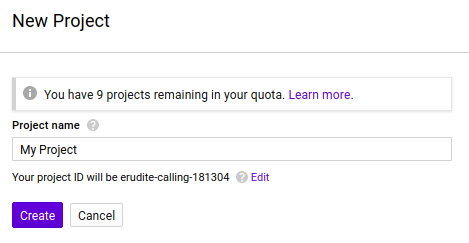
\includegraphics[width=300px, keepaspectratio]{../images/create_project.png}
		\caption{Tạo một project mới trên Google API Console.}
	\end{figure}
	\item Kích hoạt dịch vụ Google Maps JavaScript API.
\end{enumerate}

\section{Lấy API keys}

\begin{enumerate}
	\item Truy cập vào Google API Console: https://console.developers.google.com 
	\item Chọn project vừa tạo ``My Project''.
	\item Từ menu bên trái, chọn ``APIs \& services'' và chọn ``Credentials''.
	\item Click vào ``Create credentials'' và chọn ``API key''.
	\item Click vào ``Restrict'' để thiết lập bảo mật cho API key. Bước này nhằm mục đích để đảm bảo rằng chỉ có ứng dụng của chúng ta mới có quyền sử dụng API key này, tránh người khác sử dụng key lậu.
\end{enumerate}

\end{document}